\documentclass{article}
\usepackage{array}
\usepackage{geometry}
\geometry{a4paper, margin=0.6in}
\usepackage{enumitem}
\usepackage{graphicx}
\usepackage{ragged2e}
\usepackage{tcolorbox}
\usepackage{palatino}


\newcommand{\emailText}[2]{
\begin{tcolorbox}[colback=yellow!10!white, colframe=black, title=#1]
\begin{quote}
#2
\end{quote}
\end{tcolorbox}
}

\title{Responses to\\ EA Test Tasks}
\author{Mohamed Moughamir}
\date{\today}

\begin{document}
% Custom Title Page

\maketitle
\newpage
\vfill
\section*{Introduction}
This document outlines my approach to the Executive Assistant test tasks provided by \textbf{ScaleJet} for the \textbf{voilechic.com CEO support role}. My responses are guided by the core principles of effective executive support: proactive anticipation of needs, efficient task management, clear and concise communication, and meticulous attention to detail.\\

My approach to each task is as follows:
\begin{enumerate}
    \item \textbf{Email Management and Prioritization:} I prioritize emails based on urgency, impact on the CEO, and consideration of their existing schedule. My responses aim to be prompt, professional, and proactive, gathering necessary information and anticipating potential follow-up actions.
    \item \textbf{Handling Personal Tasks:} I focus on efficient problem-solving, taking ownership of each task and providing the CEO with clear and concise updates. My approach emphasizes research, resourcefulness, and clear communication.
    \item \textbf{Travel Coordination:} My travel recommendations prioritize convenience, cost-effectiveness, and alignment with the CEO's preferences. I provide well-researched options with detailed information to facilitate informed decision-making.
    \item \textbf{Calendar Scheduling:} I analyze the provided schedule to identify areas for improvement, focusing on optimizing the CEO's time by introducing buffer periods, standardizing meeting lengths, and ensuring adequate breaks.
\item \textbf{Problem Solving (Proactivity Test):} I demonstrate proactive thinking by anticipating the CEO's needs during international travel, providing well-researched recommendations that align with their preferences and ensure a productive trip.
\end{enumerate}


By addressing each task with these principles in mind, I aim to demonstrate my ability to provide comprehensive and effective support as an Executive Assistant.
\vfill
\tableofcontents
\vfill
\newpage
\section{\centering Abstract} 
\justifying{
This document presents responses to an Executive Assistant test task, showcasing proficiency in key areas such as email management, task prioritization, travel coordination, and calendar optimization.\\ Actionable recommendations are provided to improve executive efficiency and support.
}

\section{Email Management and Prioritization}
\begin{enumerate}
    \item Email 1: The \textbf{CMO} has scheduled a follow-up meeting with a client about a recent project. The meeting is set for \textit{\textbf{Thursday at 3 PM EST}}.
    \item Email 2: A \textbf{travel agent} needs confirmation of the CEO's personal vacation booking details by \textbf{tomorrow}.
    \item Email 3: The \textbf{CEO’s family member} has requested assistance in scheduling a doctor’s appointment for \textbf{tomorrow morning}.
\end{enumerate}

\subsection{Prioritization Rationale}
\paragraph{Given the analysis of the \textbf{CEO's calendar}, which revealed a consistently packed schedule with limited buffer time, the email prioritization should be adjusted to proactively manage the CEO's workload and prevent potential bottlenecks:}
\begin{enumerate}
    \item \textbf{Email 3: (CEO's family member - doctor's appointment):} This remains the \textbf{highest priority}. The time-sensitive nature (\textbf{tomorrow morning}) is critical, and securing this appointment will likely require immediate action to find an available slot, especially given the CEO's busy schedule. Failing to address this quickly could lead to significant personal disruption for the CEO.
    \item \textbf{Email 2: (Travel agent - vacation booking):} This stays as the \textbf{second priority}. While it's a personal task, the "\textbf{tomorrow}" deadline is firm. Delaying confirmation could lead to issues with the \textbf{booking and impact the CEO's personal time}, which is essential for \textbf{well-being}, \textbf{indirectly affecting their work performance}.
    \item \textbf{Email 1: (CMO - client follow-up meeting):} This moves up to the \textbf{third priority}, becoming more urgent than initially assessed. The reason for this shift is the consistently packed calendar. Even though the meeting is on Thursday, the lack of buffer time in the CEO's schedule means any preparation needed for this client meeting will need to be factored in and managed proactively. Addressing this email sooner allows for:
\begin{enumerate}
    \item Identifying any required pre-meeting tasks for the CEO.
    \item Potentially flagging any scheduling conflicts that might arise given the existing heavy load.
    \item Ensuring the CEO has ample time to prepare mentally for the follow-up.
\end{enumerate}
    

 
\end{enumerate}
\subsection{Email Responses}
\subsubsection{\textbf{Response to Email 3 (CEO’s family member):}}
\emailText{
Re: Doctor's Appointment Scheduling
}
{
Dear [CEO's Family Member's Name],\\

I'm writing to assist with scheduling the doctor's appointment for tomorrow morning. To help me find a suitable time and location, could you please provide the following information:\\

\begin{itemize}
    \item Preferred medical specialty (if applicable)
    \item General location preference (if any)
    \item Any time constraints within the morning
\end{itemize}

Once I have this information, I will contact relevant clinics/doctors and provide you with available options for your consideration.\\

Sincerely,\\

Mohamed Moughamir\\
Executive Assistant to the CEO
}

\subsubsection{\textbf{Response to Email 2 (Travel agent):}}
\emailText{Re: CEO's Personal Vacation Booking Confirmation}{
Dear [Travel Agent Name],\\

Thank you for the reminder. I will confirm the CEO's personal vacation booking details and get back to you with the confirmation by the end of today to meet your deadline.\\

Sincerely,\\

Mohamed Moughamir\\
Executive Assistant to the CEO
}

\subsubsection{\textbf{Response to Email 1 (CMO):}}
\emailText{
Re: Follow-up Meeting with Client - Thursday 3 PM EST
}{
Dear [CMO's Name],\\

Thank you for scheduling the follow-up meeting. Please let me know if you require any assistance in preparing for this meeting, such as gathering documents or setting up the meeting space (virtual or physical). I have added this to the CEO's calendar.\\

Sincerely,\\

Mohamed Moughamir\\
Executive Assistant to the CEO
}


\section{Handling Personal Tasks (Problem Solving)}

\subsection{Task 1: Amazon Return}
Steps to Resolve:
\begin{enumerate}
    \item Gather the Amazon order number, item details, and reason for return from the CEO.
    \item Access the CEO's Amazon account (with permission) to initiate the return process.
    \item Review available return options (drop-off, pickup).
    \item Schedule the return based on the CEO's preference and availability.
    \item Ensure the item is packaged appropriately.
    \item Provide the CEO with clear instructions for the return.
\end{enumerate}

\subsection{Task 2: Car Starter Repair}
Steps to Resolve:
\begin{enumerate}
    \item Obtain the car's make, model, year, and location in Canada.
    \item Identify local repair stations using online resources (Google Maps, Yelp, CAA/AAA).
    \item Utilize phone calls as the primary communication method for immediate information.
    \item Contact several repair stations to inquire about availability, estimated cost, and on-site service options.
    \item Present a summary of findings, including pricing and availability, to the CEO.
    \item Schedule the repair appointment based on the CEO's decision.
    \item Arrange for towing services if necessary.
\end{enumerate}
Communication Software: Primarily utilize direct phone calls for immediate responses. Email can be used for follow-up or when phone contact is not possible.

\subsection{WhatsApp Message to CEO}
\begin{tcolorbox}[colback=green!10!white, colframe=black, title=WhatsApp Message to CEO]
\begin{quote}
Hi [CEO's Name],\\

Just a quick update on your personal tasks:\\

\begin{itemize}
    \item \textbf{Amazon Return:} I'm gathering the necessary information to initiate the return process. I'll let you know the return options and schedule as soon as possible.
    \item \textbf{Car Repair:} I'm currently contacting local repair shops in [Location in Canada] to arrange for your car to be checked. I'll send you a summary of the available options shortly.
\end{itemize}
\end{quote}
\end{tcolorbox}

\section{Travel Coordination}
\subsection{Flight Options (Miami to New York, Arriving by 9 AM Friday)}
\begin{enumerate}
    \item \textbf{Option 1:}
    \begin{itemize}
        \item Airline: American Airlines
        \item Departure Time: 6:00 AM EST
        \item Arrival Time: 8:45 AM EST (LaGuardia Airport - LGA)
        \item Duration: 2 hours 45 minutes
        \item Total Cost: \$350 
    \end{itemize}
    \item \textbf{Option 2:}
    \begin{itemize}
        \item Airline: Delta Airlines
        \item Departure Time: 6:30 AM EST
        \item Arrival Time: 8:55 AM EST (JFK Airport)
        \item Duration: 2 hours 25 minutes
        \item Total Cost: \$380 (Example - Actual prices may vary)
    \end{itemize}
\end{enumerate}

\subsection{Hotel Options (Near Midtown Manhattan)}

\begin{enumerate}
    \item \textbf{Option 1: The Bryant Park Hotel}
    \begin{itemize}
        \item Address: 40 W 40th St, New York, NY 10018
        \item Distance from Meeting Location: Walking distance to many Midtown locations.
        \item Price per Night: \$450
        \item Total Cost (1 Night): \$450 
    \end{itemize}
    \item \textbf{Option 2: The NoMad Hotel}²
    \begin{itemize}
        \item Address: 1170 Broadway, New York, NY 10001
        \item Distance from Meeting Location: Walking distance to many Midtown locations.
        \item Price per Night: \$500 
        \item Total Cost (1 Night): \$500 
    \end{itemize}
\end{enumerate}

\section{Calendar Scheduling}

\subsection{Analysis and Suggestions for Improvement}

\begin{figure}[h]
    \centering
    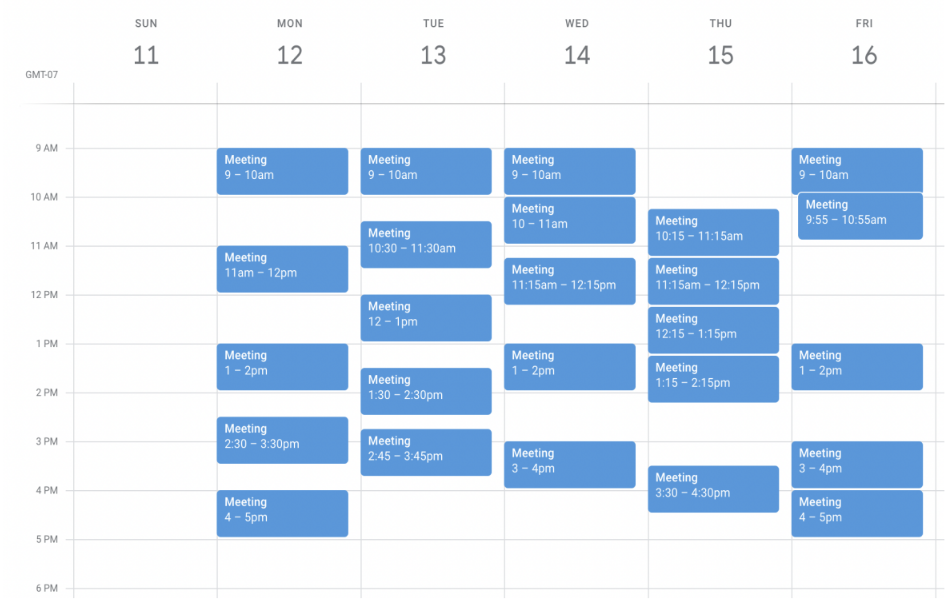
\includegraphics[width=0.6\textwidth]{unnamed.png}
    \caption{CEO's Weekly Calendar}
\end{figure}

The provided schedule is densely packed with back-to-back meetings, lacking buffer time, breaks, and consistent meeting lengths. This can negatively impact the CEO's focus, productivity, and overall well-being.\\

\textbf{Key Issues:}

\begin{itemize}
    \item \textbf{Lack of Buffer Time:} Consecutive meetings without breaks prevent the CEO from preparing, following up, or handling urgent matters.
    \item \textbf{Inconsistent Meeting Lengths:} The mix of 1-hour and shorter meetings makes scheduling and time management less efficient.
    \item \textbf{No Scheduled Breaks:} The absence of dedicated breaks can lead to burnout and reduced concentration.
    \item \textbf{Friday Meeting Overlap:} The 9:55 AM meeting on Friday overlaps with the 9:00 AM meeting, creating a scheduling conflict.
\end{itemize}

\textbf{Suggested Improvements:}

\begin{tabular}{|>{\bfseries}m{2cm}|m{11cm}|m{4cm}|} % Adjusted column widths
\hline
\textbf{Day} & \textbf{Suggested Changes} & \textbf{Rationale} \\
\hline
Monday & Introduce 15-30 minute buffer times \textit{before} the 11:00 AM meeting and \textit{after} the 2:30 PM meeting. \newline \textit{Example: 10:30-11:00 AM Buffer, 3:30-4:00 PM Buffer} & Allows for preparation, follow-up, and short breaks. \\
\hline
Tuesday & Implement 15-30 minute buffers \textit{before} the 10:30 AM and 1:30 PM meetings. Adjust the 12:00 PM meeting to allow for a dedicated lunch break (e.g., move it to 12:30 PM or later) or move it entirely to another day if possible. Reschedule the 2:45 PM meeting to start later (e.g., 3:00 PM). \newline \textit{Example: 10:00-10:30 Buffer, 1:00-1:30 Buffer, 12:30-1:30 Lunch, 3:00-4:00 Meeting} & Addresses back-to-back meetings, provides a lunch break, and prevents schedule compression. \\
\hline
Wednesday & Add a 15-30 minute buffer \textit{before} or \textit{after} the 10:00 AM meeting. Consider shifting the 11:15 AM meeting to 11:30 AM to create a more substantial break. \newline \textit{Example: 9:30-10:00 Buffer or 10:00-10:30 Buffer, 11:30-12:30 Meeting} & Provides time for preparation and a more effective break between meetings. \\
\hline
Thursday & This day requires the most significant adjustments. The back-to-back meetings from 10:15 AM to 2:15 PM are unsustainable. Introduce buffer times between \textit{each} meeting in this block. Ensure a dedicated lunch break is scheduled. Add a buffer \textit{before} the 3:30 PM meeting. \newline \textit{Example: 10:15-10:45 Meeting, 10:45-11:00 Buffer, 11:00-11:45 Meeting, 11:45-12:00 Buffer, 12:00-1:00 Lunch, 1:00-1:45 Meeting, 1:45-2:00 Buffer, 2:00-2:15 Meeting, 3:00-3:30 Buffer} & Prevents burnout, allows for transitions between meetings, and prioritizes a crucial lunch break. \\
\hline
Friday & \textbf{Reschedule the 9:55 AM meeting to a different time or day to avoid the direct overlap with the 9:00 AM meeting.} Implement 15-30 minute buffer times \textit{before} or \textit{after} the 1:00 PM and 3:00 PM meetings. \newline \textit{Example: Reschedule 9:55 Meeting, 12:30-1:00 Buffer, 3:00-3:30 Buffer} & Resolves the scheduling conflict and provides necessary buffer time. \\
\hline
\end{tabular}

\\
\textbf{Overall Improvement Strategy:}

The primary focus should be on consistently implementing buffer times (15-30 minutes), ensuring a dedicated lunch break (at least 30 minutes), correcting the overlapping meeting on Friday, and considering blocking out time for focused work or personal time for the CEO. This will result in a more balanced and productive schedule.
\vfill







\newpage
\section{Problem Solving (Proactivity Test)}

\subsection{Boutique Hotel Options in Dubai}

\begin{enumerate}
    \item \textbf{XVA Art Hotel}
    \begin{itemize}
        \item Approximately \$200 per night.
        \item Location: Al Fahidi Historical Neighbourhood 
        \item Amenities: Free Wi-Fi, art gallery, courtyard café
        \item \textbf{Description:} XVA Art Hotel is a charming boutique hotel located in the heart of Dubai's historic Al Fahidi neighborhood. It features individually designed rooms, an art gallery showcasing contemporary Middle Eastern art, and a peaceful courtyard café. The hotel's unique blend of art and culture provides a memorable stay for guests
    \end{itemize}
    \item \textbf{Manzil Downtown}
    \begin{itemize}
        \item Price: Approximately \$250 / night
        \item Location: Downtown Dubai.
        \item Amenities: Free Wi-Fi, rooftop pool, fitness center
        \item Description: Manzil Downtown is a stylish boutique hotel situated in the vibrant Downtown Dubai area. It offers modern amenities, including a rooftop pool with stunning views of the city, a well-equipped fitness center, and a variety of dining options. The hotel's central location makes it convenient for exploring Dubai's attractions
    \end{itemize}
\end{enumerate}

\subsection*{Recommendation}
I recommend the \textbf{Manzil Downtown} as the best fit for the CEO's needs. Its central location in the business district, combined with its excellent business amenities, including reliable high-speed Wi-Fi (essential for conducting virtual meetings and staying connected with the office), a 24-hour business center, makes it ideal for a business trip.

\subsubsection*{Note}
Boutique Hotels were aggregated with CoPilot from https://boutiquehotel.me
\end{document}